\documentclass[11pt,a4paper]{article}
\usepackage{graphicx}
\usepackage{float}
\usepackage{booktabs}
\usepackage{geometry}
\usepackage{hyperref}
\geometry{margin=1in}
\usepackage{tikz}
\usetikzlibrary{shapes,arrows,positioning}




\begin{document}

%-------

%--------

\section*{Network Topology Overview}
This section illustrates the network topologies used in the experiments. Each diagram explicitly shows network namespaces, their individual interfaces, and the virtual Ethernet (veth) connections between them.

\subsection*{Layer-3 Routed Topology}

\begin{figure}[H]
\centering
\begin{tikzpicture}[
    box/.style={draw, rounded corners, minimum width=3.8cm, minimum height=1.6cm, align=left},
    iface/.style={font=\small},
    link/.style={-Latex, thick},
    node distance=3.2cm
]

\node[box] (ns1) {
\textbf{Namespace ns1}\\
\texttt{veth-ns1}\\
10.0.1.2/24
};

\node[box, right=of ns1] (router) {
\textbf{Router Namespace}\\
\texttt{veth-r1} : 10.0.1.1/24\\
\texttt{veth-r2} : 10.0.2.1/24
};

\node[box, right=of router] (ns2) {
\textbf{Namespace ns2}\\
\texttt{veth-ns2}\\
10.0.2.2/24
};

\draw[link] (ns1.east) -- node[above, font=\small]{veth-ns1 $\leftrightarrow$ veth-r1} (router.west);
\draw[link] (router.east) -- node[above, font=\small]{veth-r2 $\leftrightarrow$ veth-ns2} (ns2.west);

\end{tikzpicture}
\caption{Layer-3 routed topology showing explicit interfaces in each namespace}
\end{figure}

\subsection*{Layer-2 Linux Bridge Topology}

\begin{figure}[H]
\centering
\begin{tikzpicture}[
    box/.style={draw, rounded corners, minimum width=3.8cm, minimum height=1.4cm, align=left},
    bridge/.style={draw, rounded corners, minimum width=4.2cm, minimum height=1.2cm, align=center},
    link/.style={-Latex, thick},
    node distance=3cm
]

\node[box] (ns1) {
\textbf{Namespace ns1}\\
\texttt{veth-ns1}\\
192.168.1.2/24
};

\node[bridge, below=of ns1] (br) {
\textbf{Linux Bridge br0}
};

\node[box, right=of ns1] (ns2) {
\textbf{Namespace ns2}\\
\texttt{veth-ns2}\\
192.168.1.3/24
};

\draw[link] (ns1.south) -- node[left, font=\small]{veth-ns1 $\leftrightarrow$ veth-br1} (br.north);
\draw[link] (ns2.south) -- node[right, font=\small]{veth-ns2 $\leftrightarrow$ veth-br2} (br.north);

\end{tikzpicture}
\caption{Layer-2 Linux bridge topology with explicit veth endpoints}
\end{figure}

\subsection*{Layer-2 Open vSwitch Topology}

\begin{figure}[H]
\centering
\begin{tikzpicture}[
    box/.style={draw, rounded corners, minimum width=3.8cm, minimum height=1.3cm, align=left},
    ovs/.style={draw, rounded corners, minimum width=4.4cm, minimum height=1.3cm, align=center},
    link/.style={-Latex, thick},
    node distance=3cm
]

\node[box] (ns1) {
\textbf{Namespace ns1}\\
\texttt{veth-ns1}
};

\node[ovs, below=of ns1] (ovsbr) {
\textbf{Open vSwitch}\\
\texttt{ovs-br0}
};

\node[box, right=of ns1] (ns2) {
\textbf{Namespace ns2}\\
\texttt{veth-ns2}
};

\draw[link] (ns1.south) -- node[left, font=\small]{veth-ns1 $\leftrightarrow$ veth-br1} (ovsbr.north);
\draw[link] (ns2.south) -- node[right, font=\small]{veth-ns2 $\leftrightarrow$ veth-br2} (ovsbr.north);

\end{tikzpicture}
\caption{Layer-2 topology using Open vSwitch with explicit veth endpoints}
\end{figure}


\subsection*{Detailed Namespace and veth Pair Structure}

\begin{figure}[H]
\centering
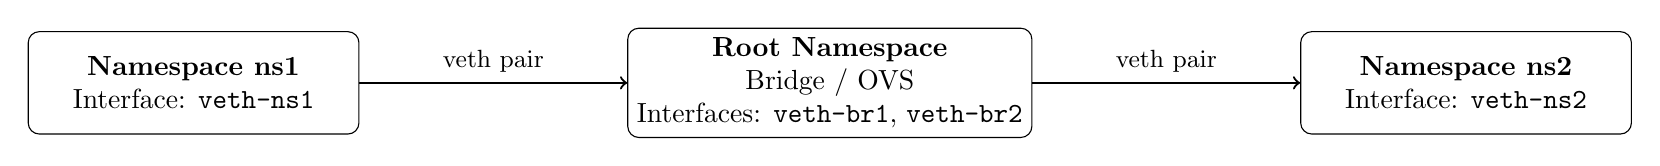
\begin{tikzpicture}[
    box/.style={draw, rounded corners, minimum width=4.2cm, minimum height=1.3cm, align=center},
    link/.style={->, thick},,
    node distance=3.4cm
]

\node[box] (ns1) {
\textbf{Namespace ns1}\\
Interface: \texttt{veth-ns1}
};

\node[box, right=of ns1] (root) {
\textbf{Root Namespace}\\
Bridge / OVS\\
Interfaces: \texttt{veth-br1}, \texttt{veth-br2}
};

\node[box, right=of root] (ns2) {
\textbf{Namespace ns2}\\
Interface: \texttt{veth-ns2}
};

\draw[link] (ns1.east) -- node[above, font=\small]{veth pair} (root.west);
\draw[link] (root.east) -- node[above, font=\small]{veth pair} (ns2.west);

\end{tikzpicture}
\caption{Explicit relationship between namespaces, veth endpoints, and switching entities}
\end{figure}


\section*{Exercise 1: Namespace Isolation}

\subsection*{Objective}
To demonstrate network isolation using Linux network namespaces despite a shared kernel.

\subsection*{Observations}
Each namespace contains its own isolated set of network interfaces.

\begin{table}[H]
\centering
\begin{tabular}{ll}
\toprule
\textbf{Namespace} & \textbf{Interfaces} \\
\midrule
ns1 & lo, veth-ns1 \\
ns2 & lo, veth-ns2 \\
router & lo, veth-r1, veth-r2 \\
\bottomrule
\end{tabular}
\caption{Interfaces visible inside each namespace}
\end{table}

\begin{figure}[H]
\centering
\includegraphics[width=0.8\textwidth]{ex1_ns1_interfaces.png}
\caption{Interfaces inside ns1,ns2,router}
\end{figure}

\subsection*{Verification of Namespace Isolation}

To verify that interfaces in one namespace are not visible in another, attempts were made to access interfaces belonging to other namespaces. The commands resulted in errors indicating that such interfaces do not exist within the current namespace context.

\begin{figure}[H]
\centering
\includegraphics[width=0.85\textwidth]{ex1_namespace_visibility_fail.png}
\caption{Attempt to access interfaces from another namespace showing isolation}
\end{figure}

This confirms that each network namespace has a strictly isolated view of network interfaces, and interfaces are only visible within the namespace to which they are explicitly assigned.


\subsection*{Explanation}
Network namespace isolation is achieved by maintaining separate instances of the network stack within the same Linux kernel. Each namespace has its own interfaces, routing tables, ARP cache, and firewall rules. The kernel internally associates networking objects with a namespace identifier, ensuring processes can only access resources within their namespace. Communication between namespaces is possible only through explicitly created virtual interfaces such as veth pairs.

\subsection*{Summary of Namespace Isolation}

\begin{table}[H]
\centering
\begin{tabular}{ll}
\toprule
\textbf{Aspect} & \textbf{Namespace Behavior} \\
\midrule
Kernel & Shared among all namespaces \\
Network interfaces & Isolated per namespace \\
Routing tables & Separate for each namespace \\
ARP cache & Separate for each namespace \\
Firewall rules & Namespace-specific \\
Interface visibility & Restricted to owning namespace \\
Inter-namespace communication & Only via veth pairs \\
\bottomrule
\end{tabular}
\caption{Summary of network namespace isolation behavior}
\end{table}

---

\section*{Exercise 2: veth Pair Semantics}

\subsection*{Objective}
To demonstrate that veth pairs behave like physical Ethernet cables.

\subsection*{Experiment}
The router-side interface \texttt{veth-r1} was brought down, and connectivity from ns1 was tested.

\begin{figure}[H]
\centering
\includegraphics[width=0.85\textwidth]{ex2_veth_down_ping_fail.png}
\caption{Ping failure after bringing veth-r1 down}
\end{figure}

\subsection*{Restoring Connectivity}

After bringing the router-side interface back up, connectivity was immediately restored, confirming the physical-link-like behavior of veth pairs.

\begin{figure}[H]
\centering
\includegraphics[width=0.85\textwidth]{ex2_veth_up_ping_success.png}
\caption{Ping success after bringing veth-r1 back up}
\end{figure}


\subsection*{Explanation}
A veth pair consists of two tightly coupled virtual interfaces. Packets transmitted on one end immediately appear on the peer interface. When either end is brought down, the link is effectively broken, preventing communication in both directions. This behavior closely mirrors that of a physical Ethernet cable.

---

\section*{Exercise 3: Layer 2 vs Layer 3 Forwarding}

\subsection*{Objective}
To compare packet forwarding behavior in bridged (L2) and routed (L3) setups.

\subsection*{Observations}

\begin{table}[H]
\centering
\begin{tabular}{lll}
\toprule
\textbf{Aspect} & \textbf{Layer 2 (Bridge)} & \textbf{Layer 3 (Router)} \\
\midrule
Forwarding basis & MAC address & IP address \\
IP forwarding required & No & Yes \\
Same subnet required & Yes & No \\
Effect of disabling IP forwarding & No impact & Connectivity fails \\
\bottomrule
\end{tabular}
\caption{Comparison of L2 and L3 forwarding}
\end{table}

\subsection*{L3 Forwarding with IP Forwarding Disabled}

When IP forwarding was disabled in the router namespace, the routed (Layer-3) setup failed to forward packets between namespaces, even though routing tables and interfaces remained configured.

\begin{figure}[H]
\centering
\includegraphics[width=0.85\textwidth]{ex3_l3_ipforward_off_ping_fail.png}
\caption{Ping failure in L3 setup after disabling IP forwarding}
\end{figure}


\subsection*{Explanation}
In the Layer-3 routed setup, disabling IP forwarding prevents the router from forwarding packets between interfaces, breaking connectivity. In contrast, Layer-2 forwarding relies solely on MAC address learning and switching, and therefore remains unaffected by IP forwarding settings. This highlights the independence of Layer-2 forwarding from Layer-3 routing.

---

\section*{Exercise 4: Bridge MAC Learning}

\subsection*{Objective}
To observe MAC address learning and unknown unicast behavior in a Linux bridge.

\subsection*{Observations}
Before traffic generation, the forwarding database (FDB) contained no dynamic entries. After generating traffic, MAC addresses were dynamically learned.

\begin{figure}[H]
\centering
\includegraphics[width=0.85\textwidth]{ex4_fdb_empty.png}
\caption{Empty dynamic FDB before traffic}
\end{figure}

\begin{figure}[H]
\centering
\includegraphics[width=0.85\textwidth]{ex4_fdb_learned.png}
\caption{Dynamically learned MAC entries after traffic}
\end{figure}

\subsection*{Explanation}
When a bridge receives a frame with an unknown destination MAC address, it floods the frame to all ports except the incoming port. Upon receiving a response, the bridge learns the source MAC address and associates it with the corresponding port. Subsequent frames are forwarded as unicast traffic.

---

\section*{Exercise 5: Linux Bridge vs Open vSwitch}

\subsection*{Objective}
To compare throughput, CPU usage, and architecture of Linux Bridge and Open vSwitch.

\subsection*{Observations}
Throughput measurements using iperf showed comparable performance, while CPU usage was higher for Open vSwitch due to userspace components.

\subsection*{Linux Bridge Performance Measurement}

Throughput between namespaces was measured using \texttt{iperf} while connected through a Linux bridge.

\begin{figure}[H]
\centering
\includegraphics[width=0.85\textwidth]{ex5_iperf_bridge.png}
\caption{Throughput measurement using iperf over Linux bridge}
\end{figure}

CPU utilization during the test showed minimal overhead, as Linux bridge operates entirely in kernel space without dedicated userspace switching processes.

\begin{figure}[H]
\centering
\includegraphics[width=0.85\textwidth]{ex5_cpu_bridge.png}
\caption{CPU usage during iperf test over Linux bridge}
\end{figure}

\subsection*{Open vSwitch Performance Measurement}

The same throughput test was repeated after replacing the Linux bridge with Open vSwitch.

\begin{figure}[H]
\centering
\includegraphics[width=0.85\textwidth]{ex5_iperf_ovs.png}
\caption{Throughput measurement using iperf over Open vSwitch}
\end{figure}

\subsection*{CPU Usage Observation}

During the Open vSwitch experiment, additional userspace processes were observed contributing to CPU usage.

\begin{figure}[H]
\centering
\includegraphics[width=0.85\textwidth]{ex5_cpu_ovs.png}
\caption{CPU usage showing ovs-vswitchd and ovsdb-server during traffic forwarding}
\end{figure}


\begin{table}[H]
\centering
\begin{tabular}{lll}
\toprule
\textbf{Aspect} & \textbf{Linux Bridge} & \textbf{Open vSwitch} \\
\midrule
Execution space & Kernel-only & Kernel + Userspace \\
CPU usage & Low & Higher \\
SDN support & No & Yes \\
Flexibility & Limited & High \\
\bottomrule
\end{tabular}
\caption{Linux Bridge vs Open vSwitch}
\end{table}

\subsection*{Explanation}
Linux Bridge offers simple and efficient Layer-2 switching implemented entirely in kernel space. Open vSwitch uses a hybrid architecture with a kernel datapath and userspace control processes, enabling advanced features such as SDN, traffic shaping, and tunneling at the cost of increased CPU usage.

---

\section*{Exercise 6: VLAN Isolation}

\subsection*{Objective}
To demonstrate Layer-2 isolation using VLANs on a Linux bridge, even when hosts are configured with overlapping IP addresses.

\subsection*{VLAN Filtering on the Bridge}
VLAN filtering was enabled on the Linux bridge to allow logical separation of traffic at the data link layer.

\begin{figure}[H]
\centering
\includegraphics[width=0.85\textwidth]{ex6_vlan_filtering_enabled.png}
\caption{VLAN filtering enabled on the Linux bridge}
\end{figure}

\subsection*{VLAN Configuration on Bridge Ports}
Each namespace was assigned to a different VLAN on the same bridge. The namespace interfaces were configured as untagged access ports with different VLAN IDs.

\begin{figure}[H]
\centering
\includegraphics[width=0.85\textwidth]{ex6_vlan_config.png}
\caption{Bridge VLAN configuration showing different VLAN IDs assigned to each port}
\end{figure}

\subsection*{Verification of VLAN Isolation}
Both namespaces were configured with overlapping IP addresses in the same subnet. Despite this, communication between them failed due to VLAN-based Layer-2 isolation.

\begin{figure}[H]
\centering
\includegraphics[width=0.85\textwidth]{ex6_vlan_ping_fail.png}
\caption{Ping failure demonstrating VLAN-based isolation with overlapping IP addresses}
\end{figure}

\subsection*{Explanation}
VLANs partition a single physical or virtual switch into multiple logical broadcast domains. Ethernet frames belonging to one VLAN are not forwarded to ports associated with another VLAN. As a result, ARP requests do not reach hosts in different VLANs, preventing IP-level communication even when IP addresses overlap. This confirms that VLAN-based isolation is enforced at Layer 2, independent of Layer-3 addressing.


---

\section*{Exercise 7: Misconfiguration Debugging}

\subsection*{Objective}
To identify and debug a Layer-2 misconfiguration.

\subsection*{Experiment}
A namespace interface was intentionally detached from the bridge, resulting in loss of connectivity.

\subsection*{Baseline Packet Flow Observation}

Tcpdump was used to observe normal packet flow before introducing any misconfiguration.

\begin{figure}[H]
\centering
\includegraphics[width=0.85\textwidth]{ex7_tcpdump_working.png}
\caption{Tcpdump capture showing ARP and ICMP traffic in a correctly configured setup}
\end{figure}

\subsection*{Diagnosis After Misconfiguration}

After detaching one namespace from the bridge, tcpdump revealed repeated ARP requests without replies, indicating a Layer-2 failure.

\begin{figure}[H]
\centering
\includegraphics[width=0.85\textwidth]{ex7_tcpdump_broken.png}
\caption{Tcpdump capture showing repeated ARP requests without replies}
\end{figure}

\subsection*{Bridge State Verification}

The bridge configuration was inspected to confirm the misattachment of the namespace interface.

\begin{figure}[H]
\centering
\includegraphics[width=0.85\textwidth]{ex7_bridge_link_missing.png}
\caption{Bridge link output showing missing interface attachment}
\end{figure}


\subsection*{Diagnosis}
Using \texttt{bridge link}, the missing bridge attachment was identified as the root cause.

\subsection*{OSI Layer Identification}
The failure occurred at \textbf{Layer 2 (Data Link Layer)}, as Ethernet frames could not be forwarded despite correct IP configuration.

---

\section*{Exercise 8: Design Question}

\subsection*{Problem Statement}
Design an appropriate networking solution for connecting 10 containers that share a single physical network interface card (NIC), and justify the choice among VLANs, Open vSwitch (OVS), and SR-IOV.

\subsection*{Chosen Solution: Open vSwitch (OVS)}
Open vSwitch (OVS) is selected as the most suitable networking solution for connecting 10 containers sharing a single physical NIC.

\subsection*{Justification}
Open vSwitch provides a flexible, programmable, and scalable networking layer that is well suited for containerized environments. It allows multiple containers to share a single physical NIC efficiently while maintaining strong isolation and fine-grained traffic control. OVS supports advanced features such as VLAN tagging, traffic monitoring, quality of service (QoS), and software-defined networking (SDN) via OpenFlow, which are not available in plain VLAN-based solutions.

Unlike SR-IOV, Open vSwitch does not require specialized hardware support and does not impose limitations on container mobility. Containers connected via OVS remain fully compatible with Linux network namespaces, enabling easier orchestration, monitoring, and debugging. Additionally, OVS enables centralized policy enforcement and dynamic reconfiguration, which are essential in modern cloud and container orchestration platforms such as Kubernetes and OpenStack.

For a moderate-scale deployment involving 10 containers, Open vSwitch offers the best balance between performance, flexibility, manageability, and hardware independence, making it a practical and future-proof choice.

\subsection*{Comparison of Networking Options}

\begin{table}[H]
\centering
\begin{tabular}{lccc}
\toprule
\textbf{Feature} & \textbf{VLAN} & \textbf{Open vSwitch} & \textbf{SR-IOV} \\
\midrule
Hardware dependency & No & No & Yes \\
Performance & Medium & High & Very High \\
Isolation level & Layer 2 only & Layer 2/3 with policies & Hardware-level \\
SDN / OpenFlow support & No & Yes & No \\
Traffic control and QoS & Limited & Advanced & Limited \\
Scalability & Limited & High & Limited by number of VFs \\
Container portability & High & High & Low \\
Ease of management & Moderate & High & Low \\
Use in cloud platforms & Rare & Widely used & Specialized cases \\
\bottomrule
\end{tabular}
\caption{Comparison of VLAN, Open vSwitch, and SR-IOV for container networking}
\end{table}

\subsection*{Conclusion}
While VLANs provide basic Layer-2 isolation and SR-IOV delivers near bare-metal performance, Open vSwitch offers a comprehensive networking solution that balances performance with flexibility and ease of management. Its ability to integrate seamlessly with container networking stacks, support advanced traffic policies, and operate without specialized hardware makes it the most suitable choice for connecting 10 containers sharing a single physical NIC.


\end{document}
